\documentclass{article}
\usepackage[T1]{fontenc, graphicx} % Required for inserting images

\title{Dokumentacja Techniczna Programu "Labirynt"}
\author{Jakub Hamerlik i Marcel Opałko}
\date{2 Marzec 2024}

\begin{document}

\maketitle

\section{Idea działania programu}

Program pozwala na znalezienie drogi przez wczytany uprzednio labirynt, który jest plikiem tekstowym zawierającym definicje odpowiednich punktów

\begin{itemize}
    \item P - punkt wejścia do labiryntu
    \item K - punkt wyjścia z labiryntu,
    \item X - ściana labiryntu
    \item spacja - ścieżka, po której można się poruszać
\end{itemize}

W naszym programie będziemy korzystać z algorytmu DFS (Deep First Search) do znajdywania drogi przez labirynt.\newline

Maksymalny rozmiar labiryntu to 1024 x 1024 liczony po ścieżkach, a więc 2049 x 2049 jeśli chodzi o znaki. (włączając znak nowej linii)\newline

Jeśli chodzi o architekturę programu - musi być ona w maksymalnym stopniu elastyczna, ponieważ w trakcie semestru może nastąpić zmiana wymagań dot. projektu.\newline

Program w C nie powinien zużywać więcej pamięci niż 512kB w czasie całego swojego działania. Aby spełnić ten warunek, należy dobrze zarządzać pamięcią w programie, więc podejmiemy kroki:
\begin{itemize}
    \item Będziemy wczytywać labirynt kawałek po kawałku.
    \item Ograniczymy złożoność obliczeniową poprzez np. usunięcie zbędnych pętli.
    \item Brak wielokrotnego zwalniania pamięci
    \item Zapobieganie wyciekom pamięci
\end{itemize}

\newpage


Wyjściem z programu będzie lista wykonywanych kroków, np w postaci:\newline
\begin{verbatim}
        START
        FORWARD X (X = liczba kroków w przód)
        TURNLEFT
        ...
        STOP
\end{verbatim}
       

\section{Wywołanie programu}

\begin{enumerate}
    \item Skompiluj program za pomocą pliku makefile (w katalogu projektu),\newline wpisując komendę "make"
 
    \item Uruchom program, podając odpowiednie parametry wejściowe.
    \begin{verbatim}
    ./program nazwa_pliku_wejściowego nazwa_pliku_wyjściowego
    \end{verbatim}
    \begin{itemize}
    \item $nazwa\_ pliku\_wejściowego$ - nazwa pliku z którego wczytywany jest labirynt
    \item $nazwa\_ pliku\_wyjściowego$ - nazwa pliku do którego ma być zapisana ścieżka (lista) (brak podania tego argumentu skutkuje wypisaniem śćieżki na stdout)
    \end{itemize}
    
\end{enumerate}



\section{Podział programu na moduły}

Program przechodzenia labiryntu będzie dzielił się na kilka kluczowych modułów:

\begin{itemize}
\item Funkcja wczytująca dane z pliku wejściowego i zmieniająca te dane na format wygodny do użycia w reszcie programu.
\item Funkcja DFS przechodząca się po labiryncie reprezentowanego za pomocą grafu, szukająca przejścia od wejścia do wyjścia.
\item Funkcja intepretująca ścieżkę DFS na format wyjściowy, czyli listę kolejnych kroków przejścia po labiryncie.
\item Funkcja dzieląca labirynt na mniejsze części i zapisująca je w plikach chwilowych. Pozwoli to na zaoszczędzenie pamięci używanej podczas programu.
\end{itemize}

\section{Opis podstawowych funkcji i struktur}

Program zawierać będzie kilka struktur:
\begin{itemize}
\item Tablicę dwuwymiarową int’ów (T), która będzie zawierać dla każdego pola labiryntu listę pól, do których można z niego przejść. Np. dla labiryntu:
\end{itemize}

    \centering
    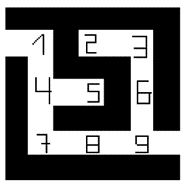
\includegraphics[width=0.3\linewidth]{image.png}


\begin{itemize}
Tablica będzie wyglądać:\newline

\item $1\{4\}, 2\{3\}, 3\{2,6\}, 4\{1,5,7\}, 5\{4\}, 6\{3,9\}, 7\{4,8\}, 8\{7,9\}, 9\{6,8\}$
\end{itemize}
\begin{itemize}
\item Tablicę jednowymiarową bool’i (odw), która będzie zawierać informację w których komórkach nasz algorytm DFS już był. 0 oznacza komórkę nieodwiedzoną, 1 odwiedzoną.
\end{itemize}

\begin{flashleft}
Oprócz struktur program zawierać będzie również funkcje:
\end{flashleft}

\begin{itemize}

\item Funkcja podziel – będzie używana w każdej innej funkcji tego programu. Będzie ona dzielić labirynt na pomniejsze kwadratowe segmenty (rozmiar każdego z nich jest jeszcze do ustalenia, przykładowo może mieć rozmiar 64x64) i zapisywać je w plikach chwilowych.

\item Funkcja wczyt – będzie przyjmować plik wejściowy i przetwarzać ten plik na format opisany  w strukturze powyżej (T).

\item Funkcja DFS – będzie używać algorytmu DFS aby przejść się po labiryncie i znaleźć w nim przejście. Funkcja będzie zapisywać ścieżkę przejścia, aby ułatwić działanie funkcji intepretującej wyniki. 

\item Funkcja wypis – będzie intepretować wyniki funkcji DFS na format wyjściowy opisany w wymogach zadania, np.:\newline
START\newline
FORWARD 1\newline
TURNLEFT\newline
FORWARD 4\newline
TURNRIGHT\newline
FORWARD 3\newline
STOP\newline
\end{itemize}



\end{document}
